\section{Experiments: Fixed NPFs, NPF Learning and Verification of Claim II}\label{sec:experiments} 
In this section, we justify ``Claim II'', i.e., active sub-networks learning is key for generalisation. Since the active sub-network are encoded in the NPFs, we verify the claim by comparing different network settings which vary in their NPF learning capabilities. We resolve the open question of \cite{arora2019exact} mentioned in \Cref{sec:background}, by providing an empirical explanation for the performance gain of finite width CNN over the pure kernel method based on the exact infinite width CNTK.\\
\textbf{Networks for Comparison:} The performance of the following networks on standard MNIST and CIFAR-10 datasets will be used for comparison: (i) fixed random (FRNPF): in the DGN, we randomly initialise both $\Tg_0,\Tv_0$, make $\Tg$ \emph{non-trainable} and train only $\Tv$ , (ii) fixed learnt (FLNPF): we initialise $\Tv_0$ randomly, and copy weights from a pre-trained ReLU network (of identical architecture) into $\Tg_0$. Similar to FR case, $\Tg$ is non-trainable and only $\Tv$ is trained (iii) decoupled learning (DNPFL):  we randomly initialise both $\Tg_0,\Tv_0$, and train both $\Tg$ and $\Tv$, (iv) ReLU: Standard DNNs/CNNs with ReLU.  We will also use the numerical results reported in \cite{arora2019exact}.\\
%The results of our experiments on CIFAR-10 (please look at the \Cref{tb:npfs} for complete results in CIFAR-10 as well as MNIST) that supports ``Claim II' can be summarised as below:
$1.$ \textbf{Finite Vs Infinite width alone is not enough to explain the performance gain of CNN:} Both FRNPF and ReLU are finite width networks. However, performance of FRNPF is  approximately $67\%$ which is worse than CNTK of \cite{arora2019exact} whose performance is $77.43\%$, and the performance of our CNN architecture with \emph{global-average-pooling} (GCONV in \Cref{tb:npfs}) is $80.34\%$. We trained FRNPF with independent initialisation (II), where $\Tg_0$ and $\Tv_0$ are statistically independent, and dependent initialisation (DI), where $\Tg_0=\Tv_0$. FRNPF (II) and FRNPF (DI) were close in our experiments (see columns $4$ and $5$ in \Cref{tb:npfs}). Further, both FRNPF (DI) and ReLU start with the same NTK matrix at initialisation. If finite width was the sole reason for the better performance then even FRNPF (II), (DI) should have performed better than CNTK in the experiments, and they did not. Thus, finite width alone does not explain the performance gain of CNN over CNTK.\\
$2.$ \textbf{NPF Learning Vs No NPF Learning  is key to explain the performance gain of CNN:} FLNPF with weights copied from a fully trained ReLU performs close to $79.68\%$ which is almost as good as ReLU's $80.43\%$ (see FLNP column in \Cref{tb:npfs}). Further, NPFs are learnt continuously during the training, and the performance gap between FRNPF and ReLU is continuous. In the case of CIFAR-10, we trained a GCONV network (parameterised by $\bar{\Theta}$) for $60$ epochs, and we obtained $6$ different weights at various \emph{stages} of the training process. Stage $1$: $\bar{\Theta}_{10}$, stage $2$: $\bar{\Theta}_{20}$, stage $3$: $\bar{\Theta}_{30}$, stage $4$: $\bar{\Theta}_{40}$, stage $5$: $\bar{\Theta}_{50}$, stage $6$: $\bar{\Theta}_{60}$. We copy these weights obtained at various stages of training to setup $6$ different FLNPFs, i.e., FLNPF-$1$ to FLNPF-$6$. We observe that the performance of FLNPF-$1$ to FLNPF-$6$ increases monotonically, with FLNPF-$1$ performing $72\%$ which is better than FRNPF (i.e., $67.08\%$),  and FLNPF-$6$ performing as well as ReLU (see left most plot in \Cref{fig:dynamics}). The performance of CNTK of \cite{arora2019exact} is $77.43\%$. Thus, through its various stages, the FLNPF starts from below $77.43\%$ and surpasses to reach $79.68\%$, which implies performance gain of CNN is due to learning of NPFs.\\
%Since from \Cref{th:main} we know that the generalisation performance of the fixed NPF learner is characterised by its NPK, and the fact that FLNPF almost recovers the performance of ReLU, we observe that \emph{almost all the information learnt by a standard ReLU DNN is stored in its gates}. 
\begin{figure}
\centering
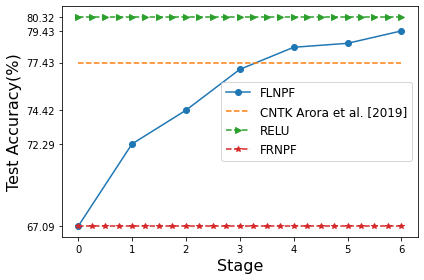
\includegraphics[scale=0.23]{figs/gap.png}
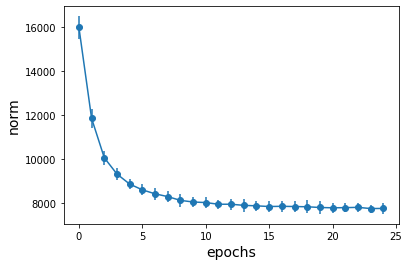
\includegraphics[scale=0.23]{figs/path-gram.png}
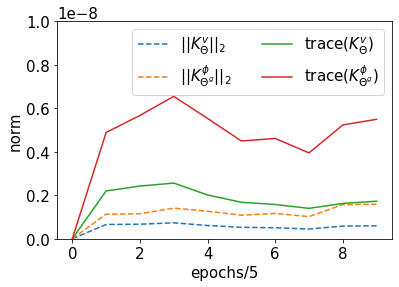
\includegraphics[scale=0.23]{figs/kvkphi.png}
\caption{Dynamics of NPF Learning. }
\label{fig:dynamics}
\end{figure}
$3.$ \textbf{Dynamics of active sub-networks during training:} We considered ``Binary''-MNIST data set with two classes namely digits $4$ and $7$, with the labels taking values in $\{-1,+1\}$ and squared loss. We trained a fully connected (FC) network ($w=100$, $d=5$). Let $\widehat{H}_{\Theta_t}=\frac{1}{trace(H_{\Theta_t})}H_{\Theta_t}$ be the normalised NPK matrix. For a subset size, $n'=200$ ($100$ examples per class) we plot $\nu_t=y^\top (\widehat{H}_{\Theta_t})^{-1} y$, (where $y\in\{-1,1\}^{200}$ is the labelling function), and observe that $\nu_t$ reduces as training proceeds (see middle plot in \Cref{fig:dynamics}). Note that, $\nu_t=\sum_{i=1}^{n'}(u_{i,t}^\top y)^2 (\hat{\rho}_{i,t})^{-1}$, where $u_{i,t}\in \R^{n'}$ are the orthonormal eigenvectors of $\widehat{H}_{\Theta_t}$ and $\hat{\rho}_{i,t},i\in[n']$ are the corresponding eigenvalues. Since $\sum_{i=1}^{n'}\hat{\rho}_{i,t}=1$, the only way $\nu_t$ reduces is when more and more energy gets concentrated on $\hat{\rho}_{i,t}$s for which $(u_{i,t}^\top y)^2$s are also high. Since $H_{\Theta_t}=\Sigma\odot \Lambda_{\Theta_t}$, only $\Lambda_{\Theta_t}$ is learnt during training.\\
$4.$ \textbf{Decoupled learning} of NPFs also performed better than FRNPFs (see column DNPFL in \Cref{tb:npfs}). This demonstrates the fact that NPFs can also be learnt in `stand alone' manner. In this case, the NTK is given by $K_{\Tdgn}=K^{\text{V}}_{\Tdgn}+K^{\text{F}}_{\Tdgn}$. For MNIST, we compared $K^{\text{V}}_{\Tdgn}$ and $K^{\text{F}}_{\Tdgn}$ (calculated using $100$ examples in total with $10$ examples per each of the $10$ classes) using their trace and Frobenius norms, and we observe that $K^{\text{V}}_{\Tdgn}$ and $K^{\text{F}}_{\Tdgn}$ are in the same scale (see right plot in \Cref{fig:dynamics}), which is perhaps pointing to the fact that both $K^{\text{F}}_{\Tdgn}$ and $K^{\text{F}}_{\Tdgn}$ are equally important for obtaining good generalisation performance. In DNPFL, we can separately study the kernel $K^{\text{F}}_{\Tdgn}$ responsible for NPF learning, an interesting future research direction.
%\FloatBarrier
 \begin{table}
\resizebox{\columnwidth}{!}{
\begin{tabular}{|c|c|c|c|c|c|c|c|}\hline
Arch			&Optimiser	&Dataset		&FRNPF (II) 			&FRNPF (DI)			&DNPFL					&FLNPF						&ReLU\\\hline
FC			&SGD		&MNIST 		&$95.85\pm0.10$		&$95.85\pm0.17$		&$97.86\pm0.11$			&$97.10\pm0.09$				&$97.85\pm0.09$\\\hline
FC			&Adam		&MNIST 		&$96.02\pm0.13$		&$96.09\pm0.12$		&$\mathbf{98.22\pm0.05}$	&$\mathbf{97.82\pm0.02}$		&$\mathbf{98.14\pm0.07}$\\\hline
VCONV		&SGD		&CIFAR-$10$	&$58.92\pm0.62$		&$58.83\pm0.27$ 		&$63.21\pm0.07$			&$63.06\pm0.73$				&$67.02\pm0.43$\\\hline
VCONV		&Adam		&CIFAR-$10$	&$64.86\pm1.18$		&$64.68\pm0.84$		&$\mathbf{69.45\pm0.76}$	&$\mathbf{71.4\pm0.47}$			&$\mathbf{72.43\pm0.54}$\\\hline
GCONV	&SGD		&CIFAR-$10$	&$67.36\pm0.56$		&$66.86\pm0.44$		&$\mathbf{74.57\pm0.43}$			&$\mathbf{78.52\pm0.39}$				&$\mathbf{78.90\pm0.37}$\\\hline
GCONV	&Adam		&CIFAR-$10$	&$67.09\pm0.58$		&$67.08\pm0.27$		&$\mathbf{77.12\pm0.19}$	&$\mathbf{79.68\pm0.32}$		&$\mathbf{80.43\pm0.35}$\\\hline
\end{tabular}
}
\caption{Shows the generalisation performance of  different NPFs learning settings. The values in the table are averaged over $5$ runs. Here, FC is a fully connected network with $w=100$ and $d=5$. VCONV and GCONV denote Vanilla CNN and CNN with GAP respectively. Please check \Cref{sec:expsetup} for details on architecture of VCONV and GCONV, and the hyper-parameters.}
\label{tb:npfs}
\end{table}
